\documentclass[10pt]{report}

\usepackage[utf8]{inputenc}
\usepackage[english]{babel}
\usepackage{graphicx}
\usepackage[pdf]{pstricks}

%Options: Sonny, Lenny, Glenn, Conny, Rejne, Bjarne, Bjornstrup
\usepackage[Sonny]{fncychap}
\usepackage{amsmath}
\usepackage[colorlinks=true, allcolors=blue]{hyperref}
\usepackage{hyperref}
\usepackage[a4paper,top=3cm,bottom=3cm,left=3cm,right=3cm]{geometry}

\graphicspath{ {imgs/} }

\title{
  {\Huge Inferring program structure from an execution trace}
}
\author{
  {Juan Francisco Martínez Vera}\\
  {\tt juan.martinez@bsc.es}
}
\date{\today}

\begin{document}
\maketitle
\tableofcontents

\chapter{Introduction}
A typical configuration for high performance machines are clusters. It means a t
eam of individual processors or multiprocessors (and lately more specific 
hardware like GPUs) working together, interconnected by a super-fast network. 
The fundamental idea behind these big machines is getting speedup by mean of
partitioning the problem and parallelize the execution. So all processors (or a 
subset) inthe cluster will be dealing with different parts of the same problem 
and communicating between them in order to end up with a solution. For example 
imagine we have a weather forecast software, in order to speedup the forecast 
we can partition the surface of the earth and hold every portion to one individual
processor. The communication will be needed because the weather will also depend 
on surroundings, so every partition will need also information of other partitions 
results.

In Computer Science the discipline in charge to drive research in this field is 
the High Performance Computing, i.e. HPC. HPC has been increasing in importance 
and nowadays can be said it is the third support of science with theory and 
mathematics. The science that can be done thanks to this big machines goes from 
earthquake predictions to the analysis of the DNA of a carcinogenic cell, from
weather forecast to material physics simulation. HPC research is not just limited
to the hardware layer but drive research in all layers in the Transformation 
Hierarchy\cite{transformationHierarchy} in figure \ref{transformationHierarchyImg}.

\begin{figure}
  \caption{Levels of transformation}
  \label{transformationHierarchyImg}
  \centering
    \includegraphics[width=120px]{transformationhierarchy.png}
\end{figure}

\begin{figure}
  \caption{Gordon Moore's prediction done in 1965}
  \label{moore-prediction}
  \centering
    \includegraphics[width=200px]{moore_prediction.png}
\end{figure}

Resources are limited and expensive, so we have to be smart and use them in an
efficient way. Improving the efficiency is not just a matter that affects to one
layer of the stack but can be applied to every one of them. For example the
tremendous evolution of the last fourty years were improvements done mostly on
circuits layer what have been following the Moore's law \cite{moore:1965}. The
manufacturers have been reducing the size of transistors by a ration of 2 every
18 months as were predicted in figure \ref{moore-prediction}. Performance improvements 
were also at microarchitecture level with
disruptive designs that allows ILP like HPS\footnote{High Performance Substrace,
what is indeed out-of-order execution with in-order retirement.}
\cite{Patt:1985:HNM:18927.18916}, speculative execution with prefetchers, 
branch prediction or even memory access value speculation,
VLIW\footnote{Very Long Instruction Word} or TLP\footnote{Thread Level
Parallelism} with multi-threading. Improvements on memory hierarchy like cache 
associativitym, non-blocking cache or trace cache. The last
big revolution affected both architecture and program layers and was the 
multicore revolution. Was specially important because until then, programmers were 
agnostics, just feel their programs went faster but now, programs have to be 
architecture aware. With this last revolution a new effort for hide machine stuff
from programmers arise and end up with programming models like OpenMP
\cite{openmp_new}, OpenACC\cite{openacc_new} or OmpSs\cite{ompss_new}. A relatively
recent example is shown is this paper \cite{Alvarez:2015:CPT:2872887.2750411}
where they are trying to automatically use the fast scraptchpad memories by
means of compilers procedures and extra hardware support instead
of let programmers to deal with this piece of hardware directly. The need to be 
always faster and faster is even more pressing in HPC that is in fact an
important science driver.

This thesis is centered on program layer\footnote{The program layer 
bring together the program itself, programming models, frameworks and libraries.}. 
This layer is the actual implementation of the algorithm, i.e. where programmers
transforms algorithm to  semantic code that can be transformed lately into
executable binary by compilers. This layer is indeed the interface between pure 
algorithm and the machine architecture. Having an efficient algorithm
mathecamically speaking is not enforcing having an efficient program 
because at algorithm level we do not care about the machine. 
The mechanism to assess the quality in terms of performance are the {\bf performance 
analysis tools} that allows to analyze and detect the bottlenecks. 
There are two main trends, by one hand we have the profilers and by other hand trace
tools. Profiler tools provide performance summaries. This summaries provides 
coarse-grain information, with low-overhead. It means that you can feel the problem 
and infer what could be the origin but the information is not enough if you want 
to be sure. For gather more detail, the other typical approach are the tracing 
tools. High accurate and detailed information can be obtained, but it needs 
more resources in terms of cpu, disk and analyst effort because more data implies 
more complexity. This demand of resources becomes worst since the capacity in 
terms of parallelism is increasing, so the number of tasks to monitor makes 
tracing by one hand hardly scalable and by the other hand tricky to analyze
because the huge quantity of data and because the increasing response times
during the interactive exploration of analysis results. 

Researchers are currently facing this two drawbacks. There are currently several
specialists driving research in the scalability field, they are trying to reduce 
the overhead of tracing in terms of time and trace sizes by mean of several 
techniques like machine learning, data-mining and so on like in 
\cite{llort2015intelligent} or by on-line compression like in
\cite{noeth2009scalatrace}. About analysis field, the complexity of the analysis 
can be overcome by adding intelligence to performance analysis tools, last 
trend is to provide an automatic smart layer that automate an important part 
of the analysis and help the analyzers in their work. Some examples of this 
research line are automatic performance analysis \cite{wolf2003automatic}, 
automatic structure extraction \cite{casas2007automatic}, phases detection 
\cite{gonzalez2013application} fundamental factors models \cite{casas2008aass}, 
automatic analysis throw deep learning \cite{simon:2017:perfdp} and so on.

This thesis is focused on the analysis field and is devoted to humbly contribute 
to ease the work of the analyzers by
automate part of the analysis. The goal of this work is to automatically detect
the internal structure of an application and correlate it with performance metrics by
mean of a post-mortem trace analysis that will help analyzers to have a general
overview about what is actually going on. So instead of deal with whole
information from the very beggining, this approach let the analyzer to figure
out to what part of the gathered information focus on, speeding up the process of
analysis. Also helps to correlate performance analysis with source code, 
since the detected application structure would be similar as
code structure and will contain source coude information that will allow to
easly pinpoint one metric to the code. The structure representation will ignore 
implementation details what therefore will contribute to faster and therefore better 
quality reports for developers. The implementation has been done also thinking 
in techniques of trace size reductions, in particular sampling, so is prepared 
for future developments where the traces do not contain the whole execution behavior.

\section{Motivation}

High performance computers becomes more complex every generation. The number of 
processors is increasing dramatically, e.g. the current number one on the Top500
 list\footnote{Top500 is the list of the top 500 most powerful high performance 
computers in the world. It is updated two times per year.} is the Sunway TaihuLight 
with 10,649,600 cores\cite{top500_2017} and the trend is even increment this
numbers because the exa-scale era. Analyze application with this quantity 
of processes with fine-grain detail becomes a really tough task when not
impossible because of the huge amount of information. The typical tools like 
visualizers are not enough. One of the major challenges is to
identify and present the hot spot. The researchers demands tools that ease the 
process of performance analysis therefore the main motivation of this work is to ease 
this analysis by means of reducing execution traces to the minimal and meaningful 
expression.

We can say that HPC applications shares a common idiosyncrasy between them. 
Mathematic solvers needs to iterate again and again until the result converge and 
simulation software are used to be programed to evolve over timesteps. So in 
general, HPC applications consists on a big outer loop that is being executed 
again and again the same code but with evolving data, i.e. SPMD\footnote{Single
Program Multiple Data} programs. Additionally this kind of workloads are used
to be burst syncrhonous, i.e. all ranks are executing computation and
communication phases in a syncrhonous manner. For these so regular executions a
relatively simple representation of the whole execution could be extracted, i.e.
the trace could be reduced to a minimum pseudo-code expression
with aggregated data for the whole loop so its somehow folding all the iterations
space. This pseudo-code expresses indeed the actual internal structure of the 
application.

There are previous works (discussed widely on section \ref{related_work})  that 
tries to represent the internal structure of an application but they are used to
use directed graphs like in \cite{aguilar2016event} or just callstack trees like
in \cite{saviankou2015cube}. The drawback of represent the application structure
just with directed graphs is that it is a so simplified view, in the referenced
case it is impossible to pinpoint a given loop (directed graph cycle) to the
actual code because the lack of callstack information. In case of the
referenced approach that uses callstacks tree, the lack of information becomes
from the fact that there is no representation for loops (although you have fuzzy
clues if you see the number of calls). In this thesis the proposal is to 
generate a pseudo-code with loop and conditional structures that can represent
be easily pinpointed to source code and additionally show aggregated metrics
that will allow the analyzer to detect the interesting parts to analyze in next
steps. So it can be understood as a sort of mix of the two approaches references
above.

Summarizing, the main motivation is to speedup the analysis process. In section
\ref{s:pt_evironment} the current analysis flow approach and how it can be
improved by using the tool proposed in this paper.

\section{Previous and related work}\label{related_work}

The problem of the analysis scalability is not faced for the first time in 
this paper but there is a previous work in what this thesis is rely and is 
supported on. Several tools are actually being used in order to ease the analyst
work. Talking about structure analysis we can split previous works into two main
subsets. By one hand we have the behavioral structure that want to expose the
different phases on an execution in terms of performance and by the other hand
the syntactic structure that provide information about the actual program
structure such as profiling.

\subsection{Behavioral structure}

If we consider the same bunch of code will behave, in general, in the same
manner it can be assumed that there is a powerful correlation between the
behavior and the code. By this way it can be said a behavioral analysis is a
side-channel analysis because indirectly the internal syntactic structure can be
betrayed. This consideration could be true in some cases but not in general. The 
main goal of the different approaches presented in this section is not
to present a syntactic but a behavioral structure. The motivation is that when
analyst deals with syntactic structure, time variations of the same functions is
hidden. This situation can appears for example when calling same function with
different parameters. For the analyst point of view could be more interesting to
have this information unfolded. Take into account that this same property can
end up identifying different parts of the code as the same phase.

Even if the goal of the approaches explained below does not match perfectly with
goal of this thesis, they provide a really useful insights as a related work.

In \cite{casas2007automatic} they propose, similarly to this paper, 
automatically extract the internal structure of an MPI application from a
Paraver tracefile and provide to analyst just representative phases. 
They rely on signal analysis for this propose. 
Their analysis consists on two main phases:
The first is to clean-up the trace by identify the perturbed regions.
Perturbed regions are those parts of the trace that has been perturbed nor by
the application nor by architecture but by external factors such that unknown
system activity or tracing package. Their clean-up phase is centered on remove
noise from tracing package, i.e. flush to disk. By building up a signal based
on flushing events and transform it by Closing morphological filter they end up
with this perturbed phases. The second phase is the identification of the
phases. It is done by means of autocorrelation and periodicity analysis of a
signal. This signal is build up from any metric like instantaneous FLOPs but the
use number of MPI point to point calls being executed. Once the period is
successfully detected the same process is done recursively on one of the
periods. This allows to have a hierarchical structure. Finally the output is
basically information about the different phases like number of iteration and
timing plus some representative cuts of the original trace. It differs on this
thesis approach basically on the fact that they extract the structure by
behavioral analysis instead of actual callstacks analysis. The main drawback is
this method is not concerning about noise from the actual application so same
phase on code can be detected as different phases, also if there is a lot of
perturbation at level of e.g. cache, depending on what metric is being used, no
structure could be detected. 

Similarly with the previous approach, in 
\cite{gonzalez2013application} is proposed to apply clustering techniques in
order to identify the different execution phases. Different parts of the
execution are considered as the same phase depending on the behavior,
so an analysis using some hardware metrics is
performed. The first phase is about reducing the complexity of the clustering by
filtering the less relevant computation burst, i.e. little bursts according
with a given threshold. In order to reduce the dimensionality the proposal is to
use two different dimension sets: The first one is Completed Instructions
against IPC\footnote{Instructions per cycle}. This configuration provides a
performance view. The second is Completed instructions against L1 and L2 cache
misses. This combination reflects the impact of the architecture on the
application structure. 

\subsection{Syntactic structure}

Syntactic structure is centered on providing the actual program code structure so
it needs to use some debug information about symbols and about the position of
the instruction in code is being executed and monitoring, i.e. the callstack.

The main interest on having the syntactic structure of an application is to be
aware about not just what but where. This is important in the process of who to
blame in code and provides insights of the actual application that with just
behavioral structure can not be presented like for example where do we have
loops and how many iterations performs.

Profile tools are used to present behavior information attached to a 
syntactic structure. Although this is a scalable
solution for performance monitoring, they are used to discard temporal order so
structures like loops are just exposed indirectly by the number of calls metric.
Additionally some sort of bottlenecks like late-sender problems are difficult to
detect without time order information. These following approaches presents the
information in a way that are in the midway between profilers and tracers. In
general starts from a huge trace and by means of summarizing and aggregating
data tries to present the minimum and meaningful information to the analyst.

In \cite{noeth2009scalatrace} they are concerning about the scalability of the
tracing part. Even if they are centered on the logging (or tracing) part their
work is really useful for this thesis purposes. They claim reductions of about a
thousand in terms of trace size just by detecting the structure of the
application, e.g. If the same thing is repeated 100 times, just saving it once
and tagging with the number of times it is executed should be enough. They
propose to use RSD (Regular Section Descriptors) to express MPI events nested
inside a loop and a sequence analysis algorithm loosely based on the SIGMA
scheme for memory analysis for detect the repetitive patterns. Their compression
is done in two phases. The first one is an intra-node compression, where the
repetitive patterns arise and the second one is inter-node merge, where all
single-node compressions are merged forming the whole application trace.
They introduce interesting concepts as calling sequence identification used for
unambiguously identify different MPI calls that lie on different code positions, 
and recursion folding signatures for dealing with recursion. Also they claim
that even if their main target is to compress traces, Scalatrace also can be
used for analyze the application structure by doing a little demo showing how it
can detect the most outer loop iterations or timesteps. One of the main
drawbacks of this approach is that the complexity of both intra-node and
inter-node compression can be of $O(n^2)$.

In the same line as the previous work, Compressed Complete Call Graphs (cCCG) are 
presented by \cite{knupfer2005construction}. It is about finding repetitive 
patterns for loosely or lossless compression but instead of at tracing time, 
over an already traced huge trace. 
This compression will allow to analyst to analyze whole huge traces 
interactively, difficult business when dealing with this amounts of information. 
CCG is basically a graph of function calls of a program so the main structure is
defined by the function call hierarchy while additional information are appended
usually as leaf nodes. The construction phase is quite simple. The trace is
traversed in a sequential manner, every time a function enter event is detected,
new node is generated and append to the current active node. The
other way around when exit function event is read, the current active node is
finalized and all information concerning to this node is presented e.g.
duration. Additionally, while constructing, the graph is compressed. The basic 
idea is to replace $n$ repeated sub-trees that are equal or similar with a 
reference to a single instance saving $n-1$ remaining copies. For similar is
understood that when comparing nodes not all properties must be equal for
example is not needed some scalar values like duration match perfectly (some
configured deviation is acceptable) but properties like function id must. They
claim main compression ration about 200 can be achieved with this approach.
Additionally this compression technique does not need to uncompress anything, the
user (or any analysis algorithm) just can traverse the graph and gather
information.

This approach improves profiling in the sense that same function with same call
path and different time behaviour is exposed to analyst but still presents a lack 
of information on the order of the execution of the different graph paths.In
\cite{aguilar2016event} they present the Event Flow Graphs (EFG) as an intent of
provide temporal order between events. In this case they are centered on
syntactic structure but just focused on MPI operations. EFG are
weighted directed graphs where every node is an MPI call and edges the
transitions between them, so the program code blocks executed between them.
Graph nodes can contain aggregate information like call duration or message size
and edges can be attached with information about CPU burst like performance
metrics like IPC additionally to the number of times the edge is traversed.
Now let's imagine we have a loop where there are three MPI calls $A$, $B$ and
$C$ and $B$ and $C$ are mutual exclusively executed so if we have 10 
iterations we have $A*10$, $B*5$ and $C*5$. In order to reconstruct the execution
we need information about in what iterations B and C have been executed.
So additionally they present temporal-EFG that introduce more
information for these cases where the execution order can not be reconstructed
with the previous EFG. They claim this technique can be used for trace
compression, application structure detection and visual performance analysis.
Following with application structure detection, what is where this thesis is
focused on, they use algorithms for cycle detection over the t-EFG (DFS-based)
and once cycles are detected the graph is transformed to a hierarchical tree
where loops and subloops are showed up. Statistics about loops can be gathered
like number of iterations, total time in loops and so on.

% Look if a possible drawback is different MPI in call are coalesced in same MPI
% call node

%In \cite{saviankou2015cube} \dots

% TODO
%- Cube
%- Selecting points of interest in traces using patterns of events

\section{Performance analysis tools environment and workflow}\label{s:pt_evironment}

%\begin{figure}
%  \caption{Current performance analysis workflow}
%  \label{currentAnalysisFlow}
%  \centering
%    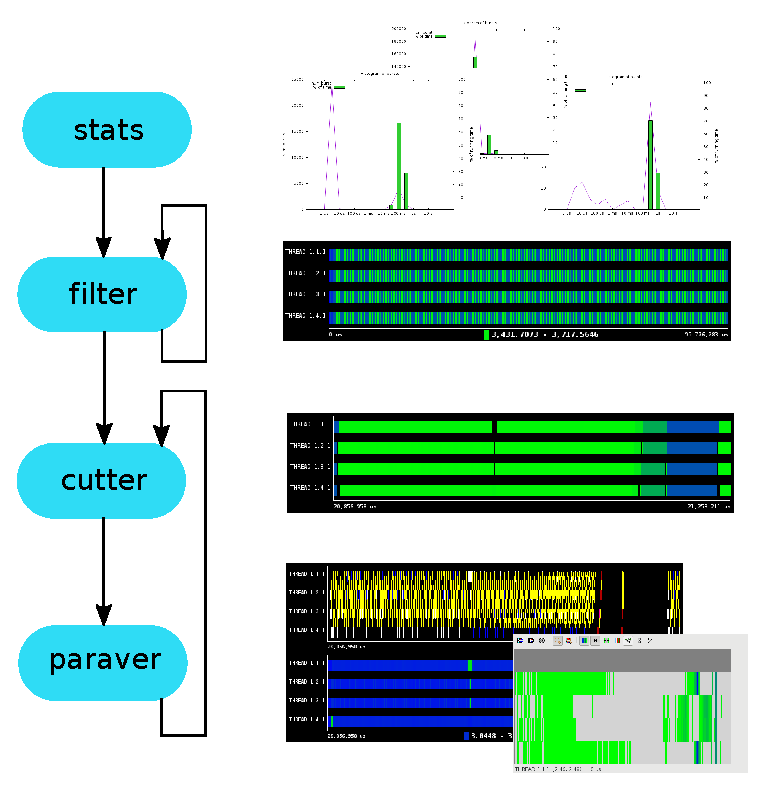
\includegraphics[width=250px]{current_analysis_flow.eps}
%\end{figure}

Talk about the BSC performance tools environment and introduce the analysis flow
with and without this proposed tool.

This is the mission of the parallel performance analysis. In an application-centric
approach, the performance analysis is a cyclic process consisting of observing 
the behaviour of the application so as to hypothesize the possible problems that 
affect its performance and finally translate these hypotheses to improvements in
the application re-starting the cycle to validate them. Obviously, the less number 
of iterations of this cycle the less time wasted and also the less money spent.


% NOTES
% .- Remember to demonstrate the interarrival time of different calls in the sam
%e loop body tend to be the same.


\bibliography{bibliography}
\bibliographystyle{apalike}
\end{document}

